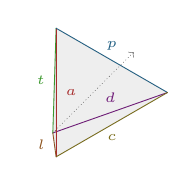
\begin{tikzpicture}[line join = round, line cap = round]
%\pgfmathsetmacro{\factor}{1/sqrt(2)};
% \coordinate [label=right:A] (A) at (2,0,-2*\factor);
% \coordinate [label=left:B] (B) at (-2,0,-2*\factor);
% \coordinate [label=above:C] (C) at (0,2,2*\factor);
% \coordinate [label=below:D] (D) at (0,-2,2*\factor);
\coordinate (A) at (0.9428090,  0.0000000, -0.3333333);
\coordinate (B) at (-0.4714045,  0.8164966, -0.3333333);
\coordinate (C) at (-0.4714045, -0.8164966, -0.3333333);
\coordinate (D) at (0.0000000,  0.0000000,  1.0000000);
% switch these to be medians (from vertex passing through opposite midpoint)
% \draw[->] (0,0) -- (3,0,0) node[right] {$x$};
% \draw[->] (0,0) -- (0,3,0) node[above] {$y$};
% \draw[->] (0,0) -- (0,0,3) node[below left] {$z$};

% median lines: pick one
% \draw[->,color={rgb:red,1;green,1;blue,1}, densely dotted, line width = {0.2pt}] (A) -- (3*-3.142697e-01, 0,  3*0.111111); % $TAL$ median
% \draw[->,color={rgb:red,1;green,1;blue,1},  densely dotted, line width = {0.2pt}] (B) -- (3*1.571348e-01,3*-2.721655e-01,3*0.1111111); % CDL median
% \draw[->,color={rgb:red,1;green,1;blue,1},  densely dotted, line width = {0.2pt}] (C) -- (3*1.571348e-01,3*2.721655e-01,3*0.1111111); % TPD median;
 \draw[->,color={rgb:red,1;green,1;blue,1},  densely dotted, line width = {0.2pt}] (D) -- (0,0,5*-0.3333333); % APC median;
 % \foreach \i in {A,B,C,D}
 %     \draw[dashed] (0,0)--(\i);
 	
 % light shaded faces
\draw[-, fill={rgb:red,1;green,1;blue,1}, opacity=.05] (A)--(D)--(B)--cycle; % TDP
\draw[-, fill={rgb:red,1;green,1;blue,1}, opacity=.05] (A)--(D)--(C)--cycle; % CDL
\draw[-, fill={rgb:red,1;green,1;blue,1}, opacity=.05] (B)--(D)--(C)--cycle; % TAL
\draw[-, fill={rgb:red,1;green,1;blue,1}, opacity=.05] (A)--(B)--(C)--cycle; % APC

% color edges
\draw[-, color ={rgb:red,136;green,31;blue,147}, line width = {0.3pt}] (A)--(D); % D
\draw[-, color ={rgb:red,197;green,117;blue,43}, line width = {0.3pt}] (D)--(C); % L
\draw[-, color ={rgb:red,78;green,201;blue,59}, line width = {0.3pt}] (D)--(B); % T
% front face
\draw[-, color ={rgb:red,210;green,55;blue,55}, line width = {0.3pt}] (B)--(C); % A
\draw[-, color ={rgb:red,49;green,145;blue,201}, line width = {0.3pt}] (A)--(B); % P
\draw[-, color ={rgb:red,210;green,188;blue,45}, line width = {0.3pt}] (A)--(C); % C

% edge labels
\node[above, color={rgb:red,49;green,145;blue,201}] at (0.2357023,  0.4082483, -0.3333333) {\tiny $p$};
\node[below, color={rgb:red,210;green,188;blue,45}] at (0.2357023, -0.4082483, -0.3333333) {\tiny$c$};
\node[above, color={rgb:red,136;green,31;blue,147}] at (0.4714045,  0.0000000,  0.3333333) {\tiny$d$};
\node[left, color={rgb:red,78;green,201;blue,59}] at (-0.2357023,  0.4082483,  0.3333333) {\tiny$t$};
\node[left, color={rgb:red,197;green,117;blue,43}] at (-0.2357023, -0.4082483,  0.3333333) {\tiny$l$};
\node[right, color={rgb:red,210;green,55;blue,55}] at (-0.4714045,  0.0000000, -0.3333333) {\tiny$a$};

% node helper labels
%\node at (A) {\small A};
% \node at (B) {\small B};
% \node at (C) {\small C};
% \node at (D) {\small D};

\end{tikzpicture}


% two versions, one with medians, another with bimedians.